\chapter{System and Methods}

\section{System Overview}

Semantic VAE is a pipeline for generating vibrotactile feedback from temporal visual events. In this thesis, the input events are represented as short UI flows consisting of three visual states: before, during, and after an interaction. These UI flows provide a controlled setting for studying a broader problem: how to translate an ordered visual change into a haptic response that has appropriate meaning, timing, and physical form. The output of the system is a two-second vibrotactile sequence that can be played on an ERM motor through the study prototype.

The system is organized around a semantic intermediate representation rather than a direct mapping from images or prompts to actuator values. Given the three visual states, the system sends the image sequence to an OpenAI 4.1 model with a schema-designed prompt, and the haptic event planner produces an ordered event plan. Each event describes the intended haptic behavior at a higher level, including its behavior class, semantic role, style, strength, timing, and duration. This representation separates the interpretation of the visual event from the synthesis of the final waveform, making it possible to inspect and revise what the system believes the haptic feedback should communicate before generating the low-level signal.

\begin{figure}[t]
\centering
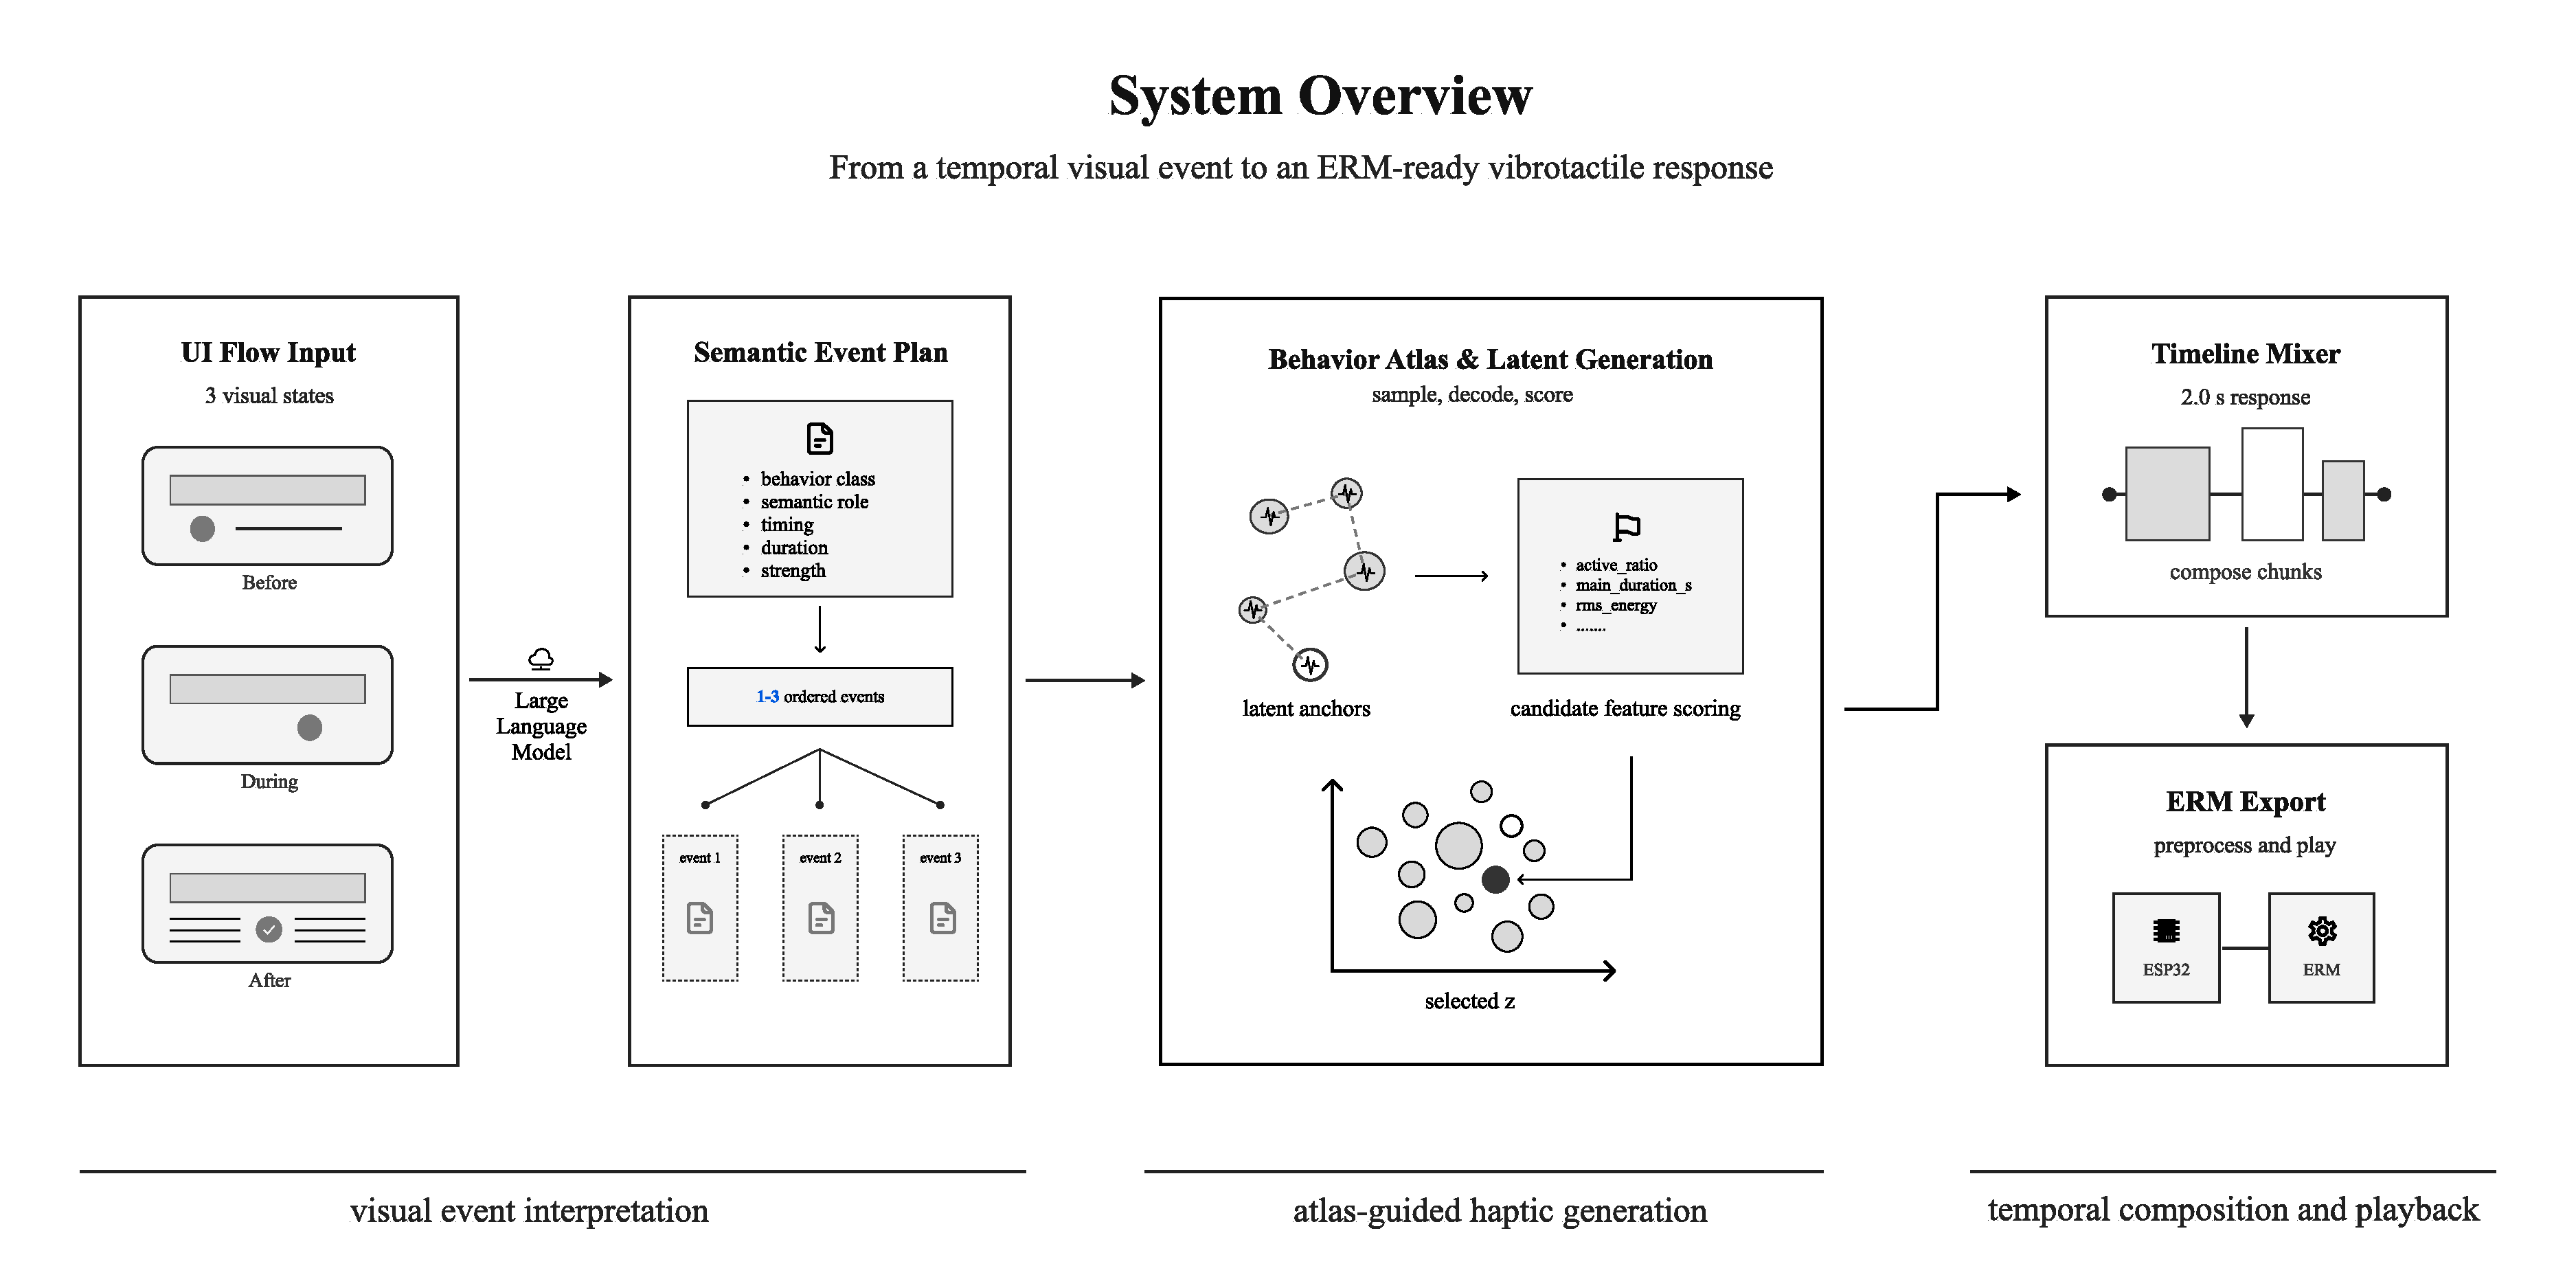
\includegraphics[width=\textwidth]{Figures/system_overview_diagram.pdf}
\caption{Semantic VAE system overview.}
\label{fig:system-overview}
\end{figure}

The event plan then guides waveform generation through a behavior atlas built over a convolutional variational autoencoder (VAE). The atlas groups learned haptic waveforms into interpretable behavior families, such as impacts, ramps, pulses, and other temporal forms. For each planned event, the system converts the semantic description into target waveform features, uses the atlas to identify a plausible region of the VAE latent space, and performs semantic-feature-guided latent search within that region.

Existing waveforms and their latent codes serve as anchors that indicate where similar haptic behaviors are located in the learned space. The system samples candidate latent vectors near those anchors, decodes each candidate with the VAE, measures the resulting waveform features, and selects the generated candidate whose decoded signal best matches the semantic target.

Generated event chunks are passed to an event timeline mixer that composes them into a coherent two-second response. This stage preserves the temporal structure of the visual event by placing each haptic chunk according to the event plan, stretching or shaping chunks as needed, and blending them into a single timeline. Finally, the composed waveform is converted into a hardware-oriented playback sequence using the same ERM preprocessing used for all study stimuli. This final stage accounts for motor constraints and produces a sequence of drive values for playback in the study prototype.

The remainder of this chapter describes each stage of the system in detail: the haptic waveform dataset and VAE model, the behavior atlas, the semantic haptic event representation, latent search, event timeline composition, and ERM export.

\section{Haptic Waveform Dataset and VAE Model}

The VAE provides the generative waveform space used by the rest of the system. It does not interpret the visual input directly. Instead, it learns a latent representation of short vibrotactile waveform chunks, and later stages use semantic planning, atlas structure, and feature-guided latent search to select generated chunks from this learned space. This separation lets the system combine learned haptic signal synthesis with explicit temporal event structure.

The model was trained on 793 WAV files from the HapticGen dataset, split into 634 training files and 159 validation files. Each file was represented during loading by an energy-rich 0.5-second segment sampled at 8 kHz, producing a 4000-sample waveform chunk. The preprocessing pipeline removes the segment mean, normalizes by a global RMS estimate, scales the result by 0.25, and clips values to the range $[-5,5]$. Min--max normalization was disabled. Lightweight augmentation was applied through random gain scaling and small temporal shifts.

\begin{figure}[t]
\centering
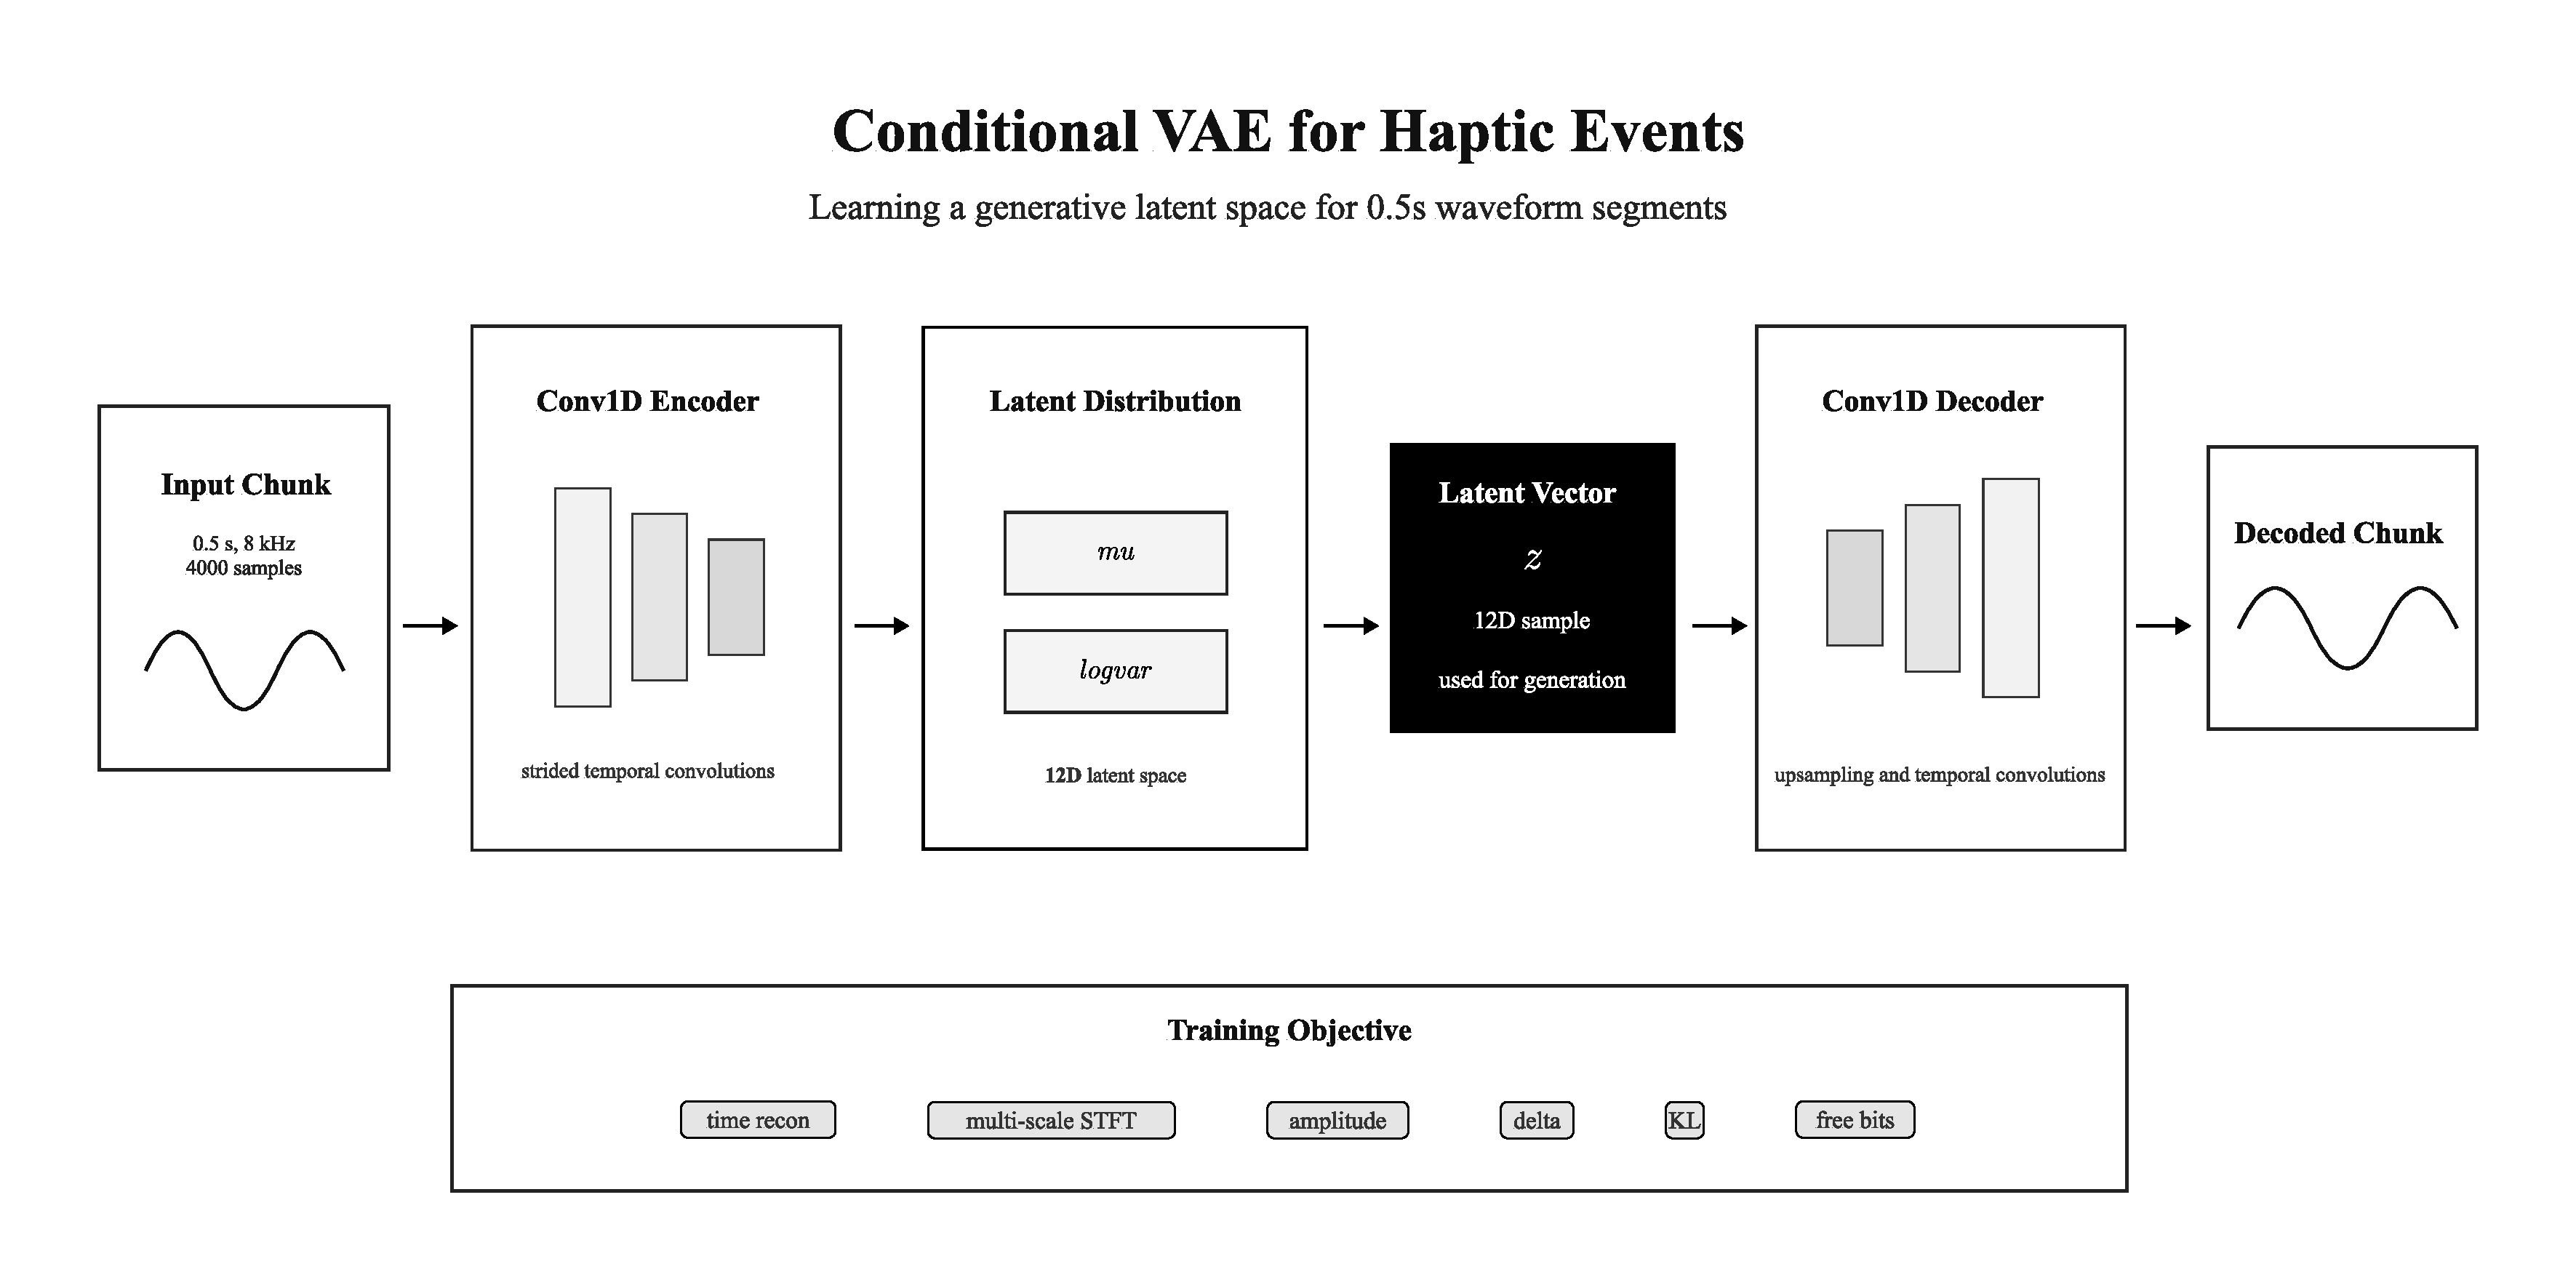
\includegraphics[width=0.95\textwidth]{Figures/conVAE_diagram.pdf}
\caption{Convolutional VAE architecture.}
\label{fig:vae-architecture}
\end{figure}

The model is a one-dimensional convolutional variational autoencoder, shown in Figure~\ref{fig:vae-architecture}. The encoder uses strided temporal convolutions to compress each waveform chunk into a 12-dimensional latent distribution parameterized by $\mu$ and $\log \sigma^2$. Latent vectors sampled from this distribution are passed to a decoder that reconstructs fixed-length waveform chunks using temporal upsampling and convolutional layers. In the generation pipeline, decoded chunks can be produced from candidate latent vectors selected by the atlas-guided search procedure described later in this chapter.

The training objective combines several terms that reflect both signal reconstruction and haptic waveform quality. Time-domain reconstruction encourages sample-level fidelity, while multi-scale STFT terms help preserve spectral structure across short and longer temporal windows. Amplitude, temporal derivative, event-envelope, local-RMS, and onset losses encourage the decoder to preserve properties that are important for vibrotactile perception, such as intensity, transient sharpness, and temporal envelope. KL regularization with free bits maintains a usable latent space for downstream sampling and search. Figure~\ref{fig:vae-training-curve} shows the training curve. Table~\ref{tab:vae-config} summarizes the VAE configuration; the full training configuration is reported in Appendix~\ref{app:system-config}.

\begin{figure}[t]
\centering
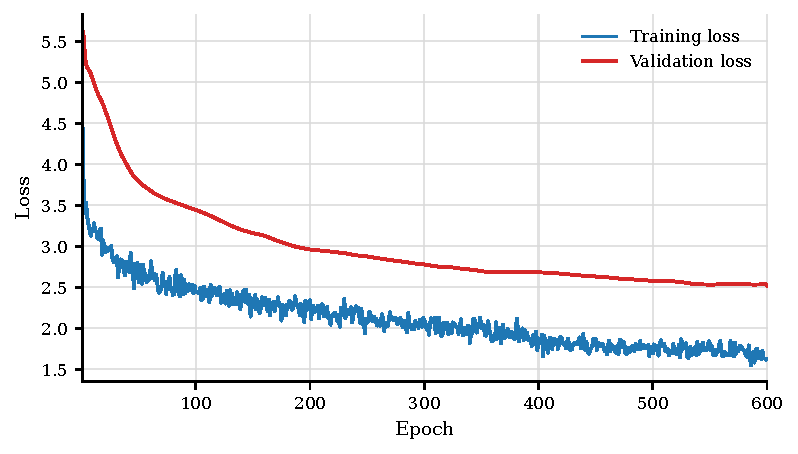
\includegraphics[width=0.78\textwidth]{Figures/vae_training_curve.pdf}
\caption{VAE training curve.}
\label{fig:vae-training-curve}
\end{figure}

\begin{table}[t]
\centering
\caption{Summary of the VAE configuration.}
\label{tab:vae-config}
\renewcommand{\arraystretch}{1.1}
\begin{tabular}{@{}>{\raggedright\arraybackslash}p{1.9in}>{\raggedright\arraybackslash}p{3.9in}@{}}
\hline
\textbf{Item} & \textbf{Configuration} \\
\hline
Dataset & 793 HapticGen WAV files \\
Split & 634 training files and 159 validation files \\
Segment & 0.5 s at 8 kHz; 4000 samples per chunk \\
Preprocessing & Energy-rich segment sampling; global RMS normalization; clipping to $[-5,5]$ \\
Model & One-dimensional convolutional VAE \\
Latent space & 12 dimensions \\
Training & 600 epochs; batch size 16 \\
Loss components & Time-domain reconstruction, multi-scale STFT, amplitude, temporal derivative, event envelope, local RMS, onset, and KL regularization \\
\hline
\end{tabular}
\end{table}


Using 0.5-second chunks rather than full two-second study stimuli is an intentional design choice. Many temporal visual events are composed of local haptic moments: an impact at the moment of confirmation, a short pulse sequence for notification, a rising or falling cue for progress, or a sustained texture for an ongoing state. Short chunks allow the VAE to learn reusable haptic units, while the timeline mixer controls how those units are placed, stretched, and combined into a complete response. The VAE therefore supplies the local generative vocabulary of the system, and later stages impose semantic and temporal structure.

\section{Behavior Atlas}

The behavior atlas organizes the VAE latent space into haptic behavior families that can be used by the semantic generation pipeline. Although the VAE learns a continuous 12-dimensional latent space, the event planner operates in semantic terms such as pulse, ramp, impact, progress, and notification. The atlas provides the bridge between these levels: it groups encoded waveform chunks into interpretable behavior categories, stores class-level latent statistics, and provides curated anchors for later latent search.

The atlas was built from the same 793 HapticGen waveform chunks used to train the VAE. Each chunk was encoded using the deterministic encoder mean $\mu$, producing a 12-dimensional latent vector for every sample. For each waveform, the atlas construction process also computed signal descriptors that capture temporal and spectral behavior, including event count, active duration, RMS energy, peak amplitude, envelope slope, late-to-early energy ratio, amplitude modulation, spectral centroid, onset density, and effective duration. These descriptors support behavior-level organization of the latent space without requiring each latent dimension to have an independent semantic interpretation.

\begin{figure}[t]
\centering
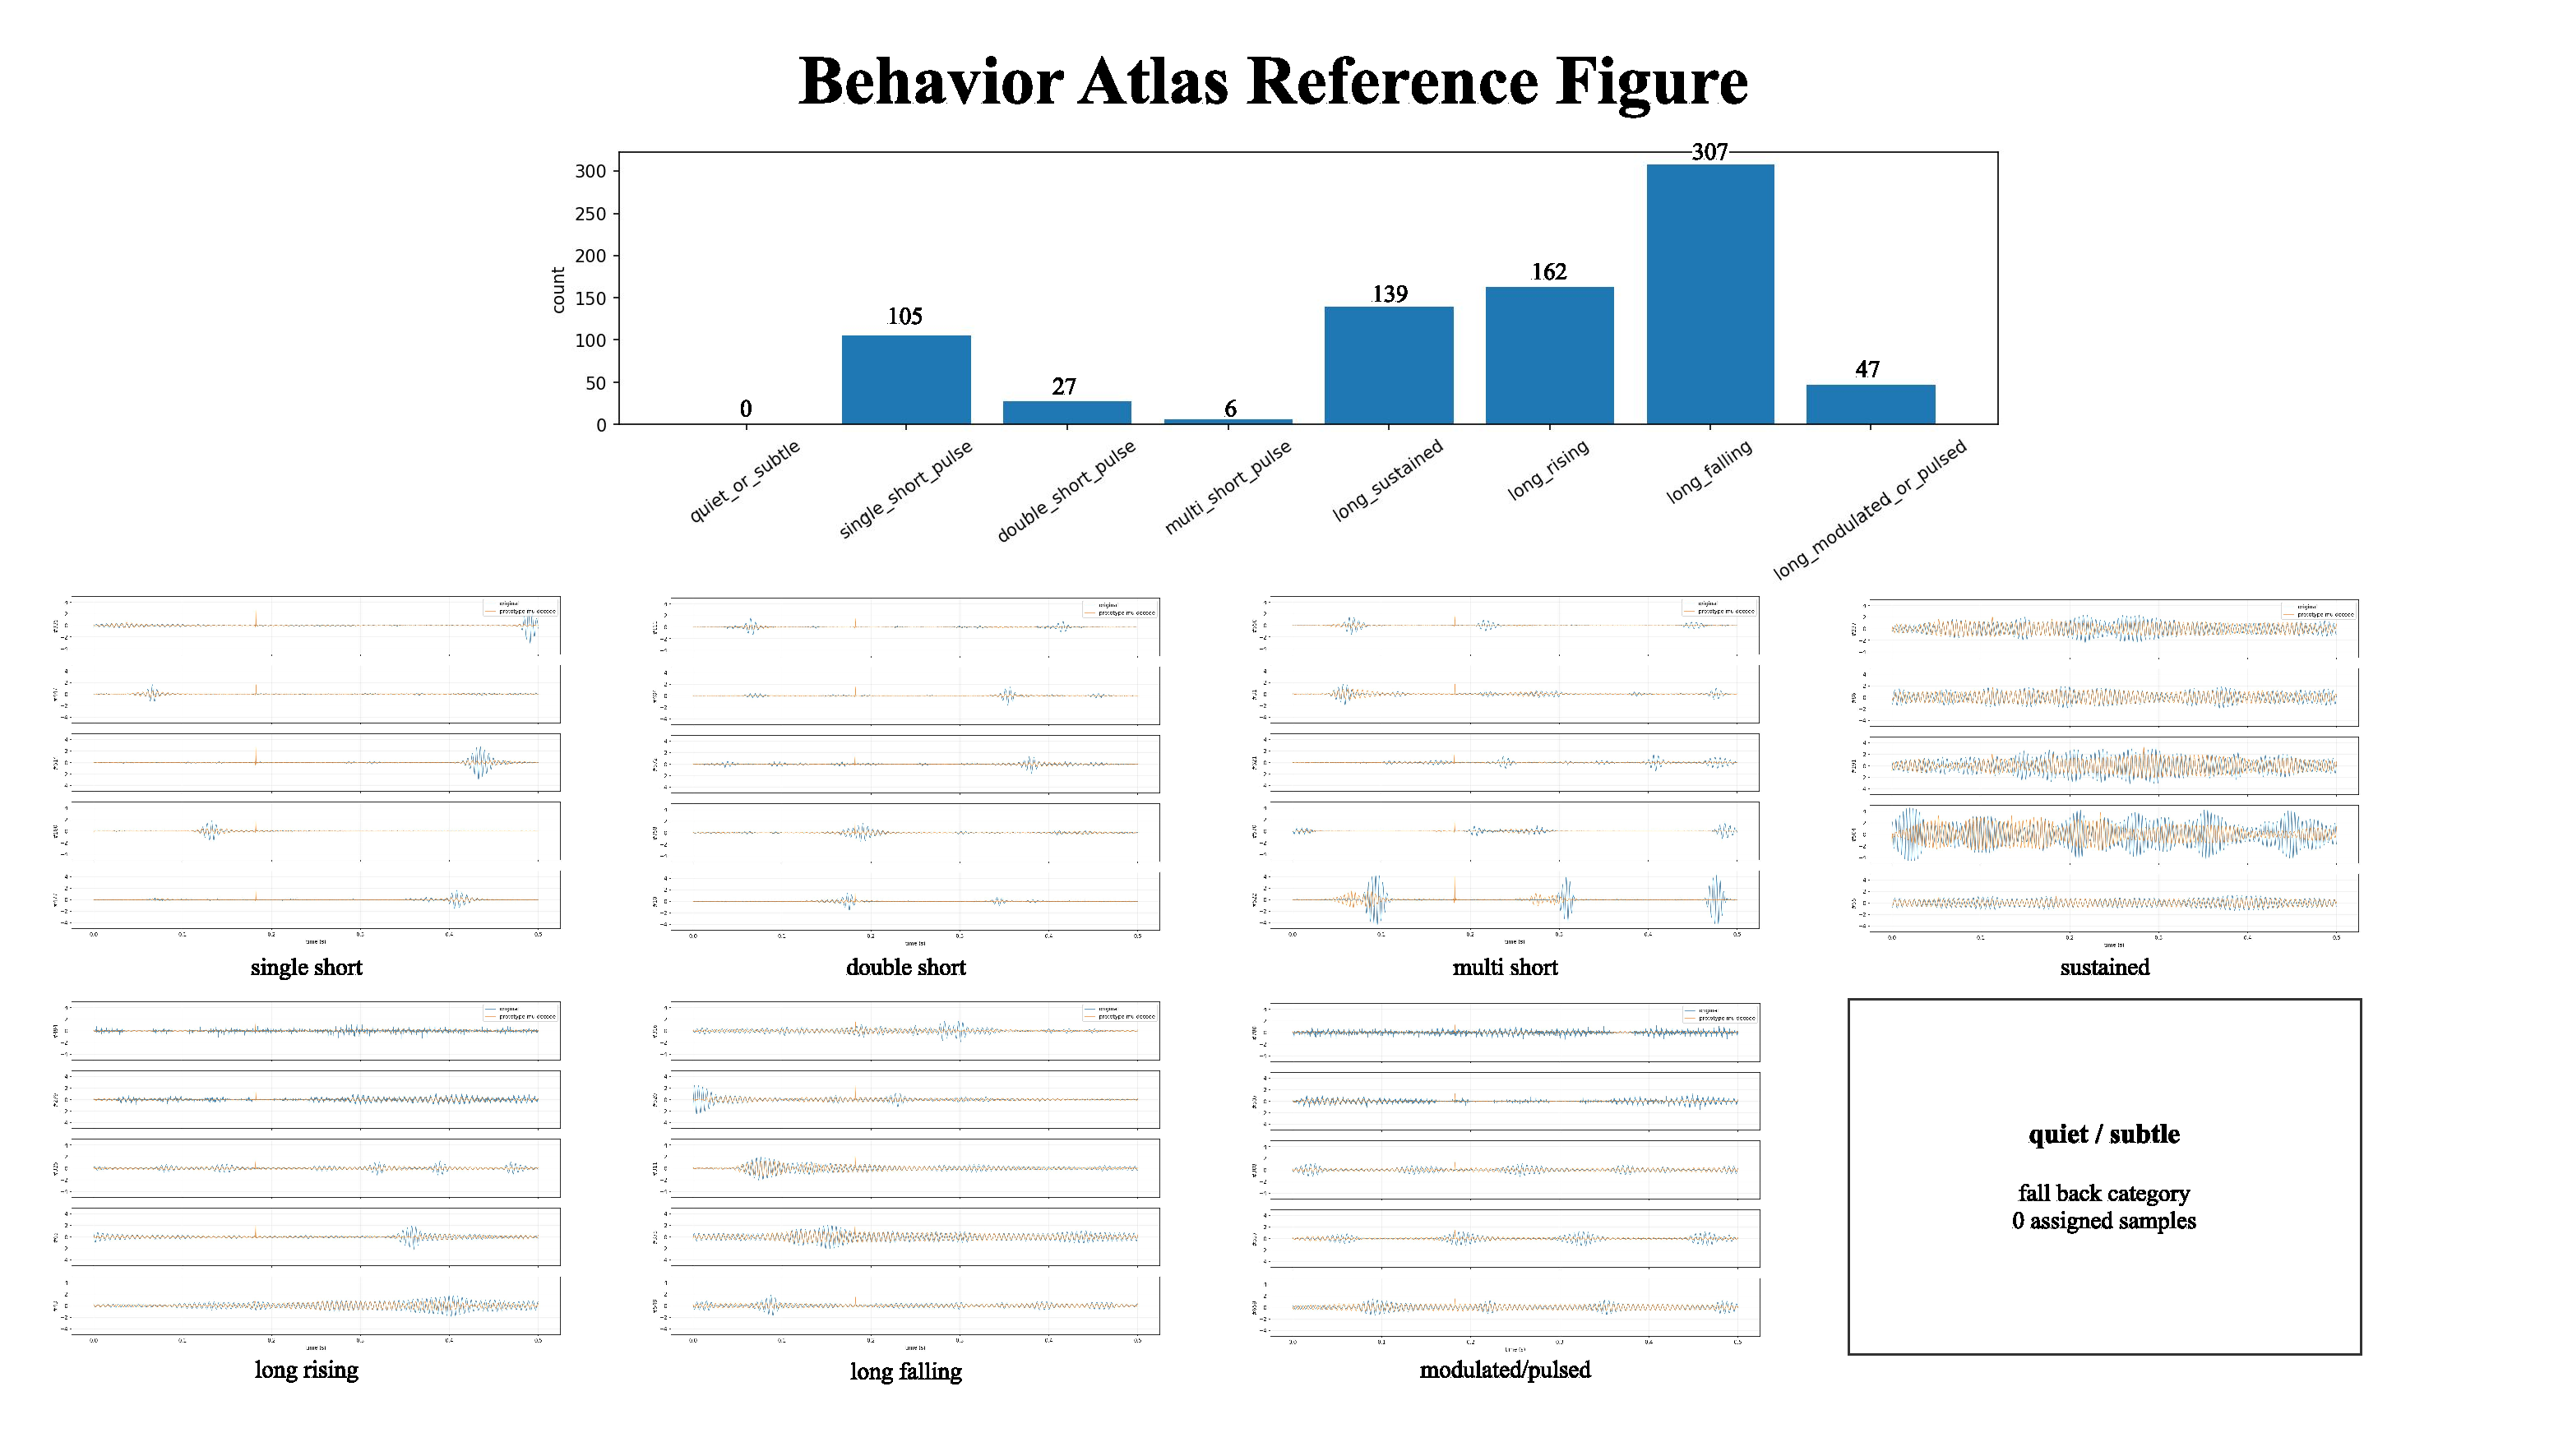
\includegraphics[width=\textwidth]{Figures/atlas_reference.pdf}
\caption{Behavior atlas.}
\label{fig:behavior-atlas}
\end{figure}

The atlas schema contains eight behavior categories: quiet or subtle, single short pulse, double short pulse, multi short pulse, long sustained, long rising, long falling, and long modulated or pulsed. Seven of these categories are represented in the final encoded dataset; quiet or subtle is retained as a fallback category for cases where the planner requests a low-intensity or minimal response. The represented classes are imbalanced, with long falling, long rising, long sustained, and single short pulse forming the largest groups, and multi short pulse appearing least often. Figure~\ref{fig:behavior-atlas} shows the class distribution and representative prototype waveforms.

After automatic feature-based organization, I manually curated the atlas prototypes used by the generation pipeline. For each represented behavior class, I selected a small set of examples that matched the intended temporal behavior. This curation was important because the latent mean of a class does not always decode to a waveform that perceptually belongs to that class. When a candidate near a class center behaved more like another category, I reassigned or excluded it from the curated prototype set. The resulting curated atlas contains two to five approved prototypes for each represented class and serves as a cleaner set of anchors for generation.

In the final system, the atlas is not used as a fixed waveform library. It provides behavior classes, latent regions, prototype anchors, and feature summaries that help the system search within the VAE latent space. When a planned haptic event specifies a behavior class, the atlas identifies a plausible region of the learned haptic manifold and supplies anchors for candidate generation. The next sections describe how the semantic event plan selects these behavior classes and how latent search generates waveform chunks from them.

\section{Semantic Haptic Event Planning}

The semantic haptic event planner converts the three visual states of a UI flow into a structured plan for haptic generation. The input consists of before, during, and after images. These images are sent in order to an OpenAI 4.1 model using a prompt designed around the event schema. The planner uses the images to identify the interaction or state change, summarize the visual transition, and choose one to three ordered haptic events. This stage represents the visual event at the level of haptic intent rather than waveform samples.

In the prototype implementation, the OpenAI 4.1 output is constrained to a fixed JSON schema rather than free-form prose. The schema defines the allowed behavior classes, semantic roles, styles, timing hints, and duration hints used by the rest of the pipeline. The planner returns a JSON object containing an interaction type, a visual change summary, optional composition notes, and an ordered list of haptic events. Each event specifies a communicative role, an atlas behavior class, a qualitative style, an intensity, a coarse timing placement, a coarse duration, and a curated prototype index used as an anchor hint. Table~\ref{tab:semantic-event-schema} summarizes the event fields.

\begin{table}[t]
\centering
\caption{Semantic haptic event schema.}
\label{tab:semantic-event-schema}
\renewcommand{\arraystretch}{1.1}
\begin{tabular}{@{}>{\raggedright\arraybackslash}p{1.45in}>{\raggedright\arraybackslash}p{4.35in}@{}}
\hline
\textbf{Field} & \textbf{Meaning} \\
\hline
\texttt{event\_type} & Visual interaction or state-change type. \\
\texttt{semantic\_role} & Communicative haptic role, such as press, drag, release, confirmation, notification, warning, state change, or subtle context. \\
\texttt{behavior\_class} & Behavior atlas category used to route the event to a latent search region. \\
\texttt{style} & Qualitative haptic style, such as soft, sharp, strong, smooth, ticked, bumpy, rising, falling, sustained, or subtle. \\
\texttt{strength} & Intended intensity on a continuous scale from 0.0 to 1.0. \\
\texttt{timing\_hint} & Coarse temporal placement: beginning, middle, or end. \\
\texttt{duration\_hint} & Coarse duration: short, medium, long, or full. \\
\texttt{prototype\_index} & Curated atlas anchor hint used by latent search. \\
\texttt{reason} & Short planner rationale for the event. \\
\hline
\end{tabular}
\end{table}


The schema uses closed option sets for the main semantic fields. Semantic roles include press-down, drag, pull, scroll, release, confirmation, notification, warning, state change, and subtle context. Style options include soft, sharp, strong, smooth, ticked, bumpy, rising, falling, sustained, and subtle. Timing hints are limited to beginning, middle, and end. Duration hints are mapped to approximate durations: short to 0.5 seconds, medium to 0.8 seconds, long to 1.2 seconds, and full to 2.0 seconds. Strength is represented as a numeric value between 0.0 and 1.0.

The planner output is intentionally higher-level than the waveform generator. It does not assign exact latent vectors or final waveform samples. Instead, it expresses what haptic behavior should occur, why it should occur, and where it should be placed within the event sequence. The prototype index is interpreted as a curated atlas anchor hint for downstream search, while the final latent vector is selected by the semantic-feature-guided search procedure described in the next section.

For example, in an error-flow stimulus where the user checks a ``Delete My Account'' option and an error modal appears, the planner produced two haptic events. The first event represented the initial press-down interaction as a sharp single short pulse at the beginning of the timeline. The second represented the later error state change as a stronger double short pulse near the end. This plan preserves the temporal structure of the visual event before waveform generation: an initial input action followed by a later system response.

Although this thesis uses UI flows as the controlled input domain, the planner is the main domain-specific component of the pipeline. Other temporal visual event domains could use the same downstream VAE, atlas, latent search, and timeline mixer if their visual events are mapped into the same semantic haptic event representation or an adapted schema.

\section{Semantic-Feature-Guided Latent Search}

Each semantic haptic event is converted into a generated latent vector through a feature-based search. The event plan defines the intended haptic behavior, the atlas locates relevant regions of the VAE latent space, and decoded waveform features determine the final candidate. Implementation parameters for this stage are reported in Appendix~\ref{app:system-config}.

The search begins by converting the event fields into target waveform features. Given a semantic haptic event $e$, the system constructs an event-derived target vector

\begin{equation}
\mathbf{t} = g(e).
\end{equation}

This target vector is initialized from the feature statistics of the requested behavior class and then adjusted according to the semantic role, style, strength, and duration hint. The target features include event count, active ratio, main event duration, RMS energy, crest factor, amplitude modulation, envelope slope, envelope decay, and spectral centroid. For example, a double short pulse event encourages two active events, while a strong or sharp style increases target energy, crest factor, and spectral centroid.

\begin{figure}[t]
\centering
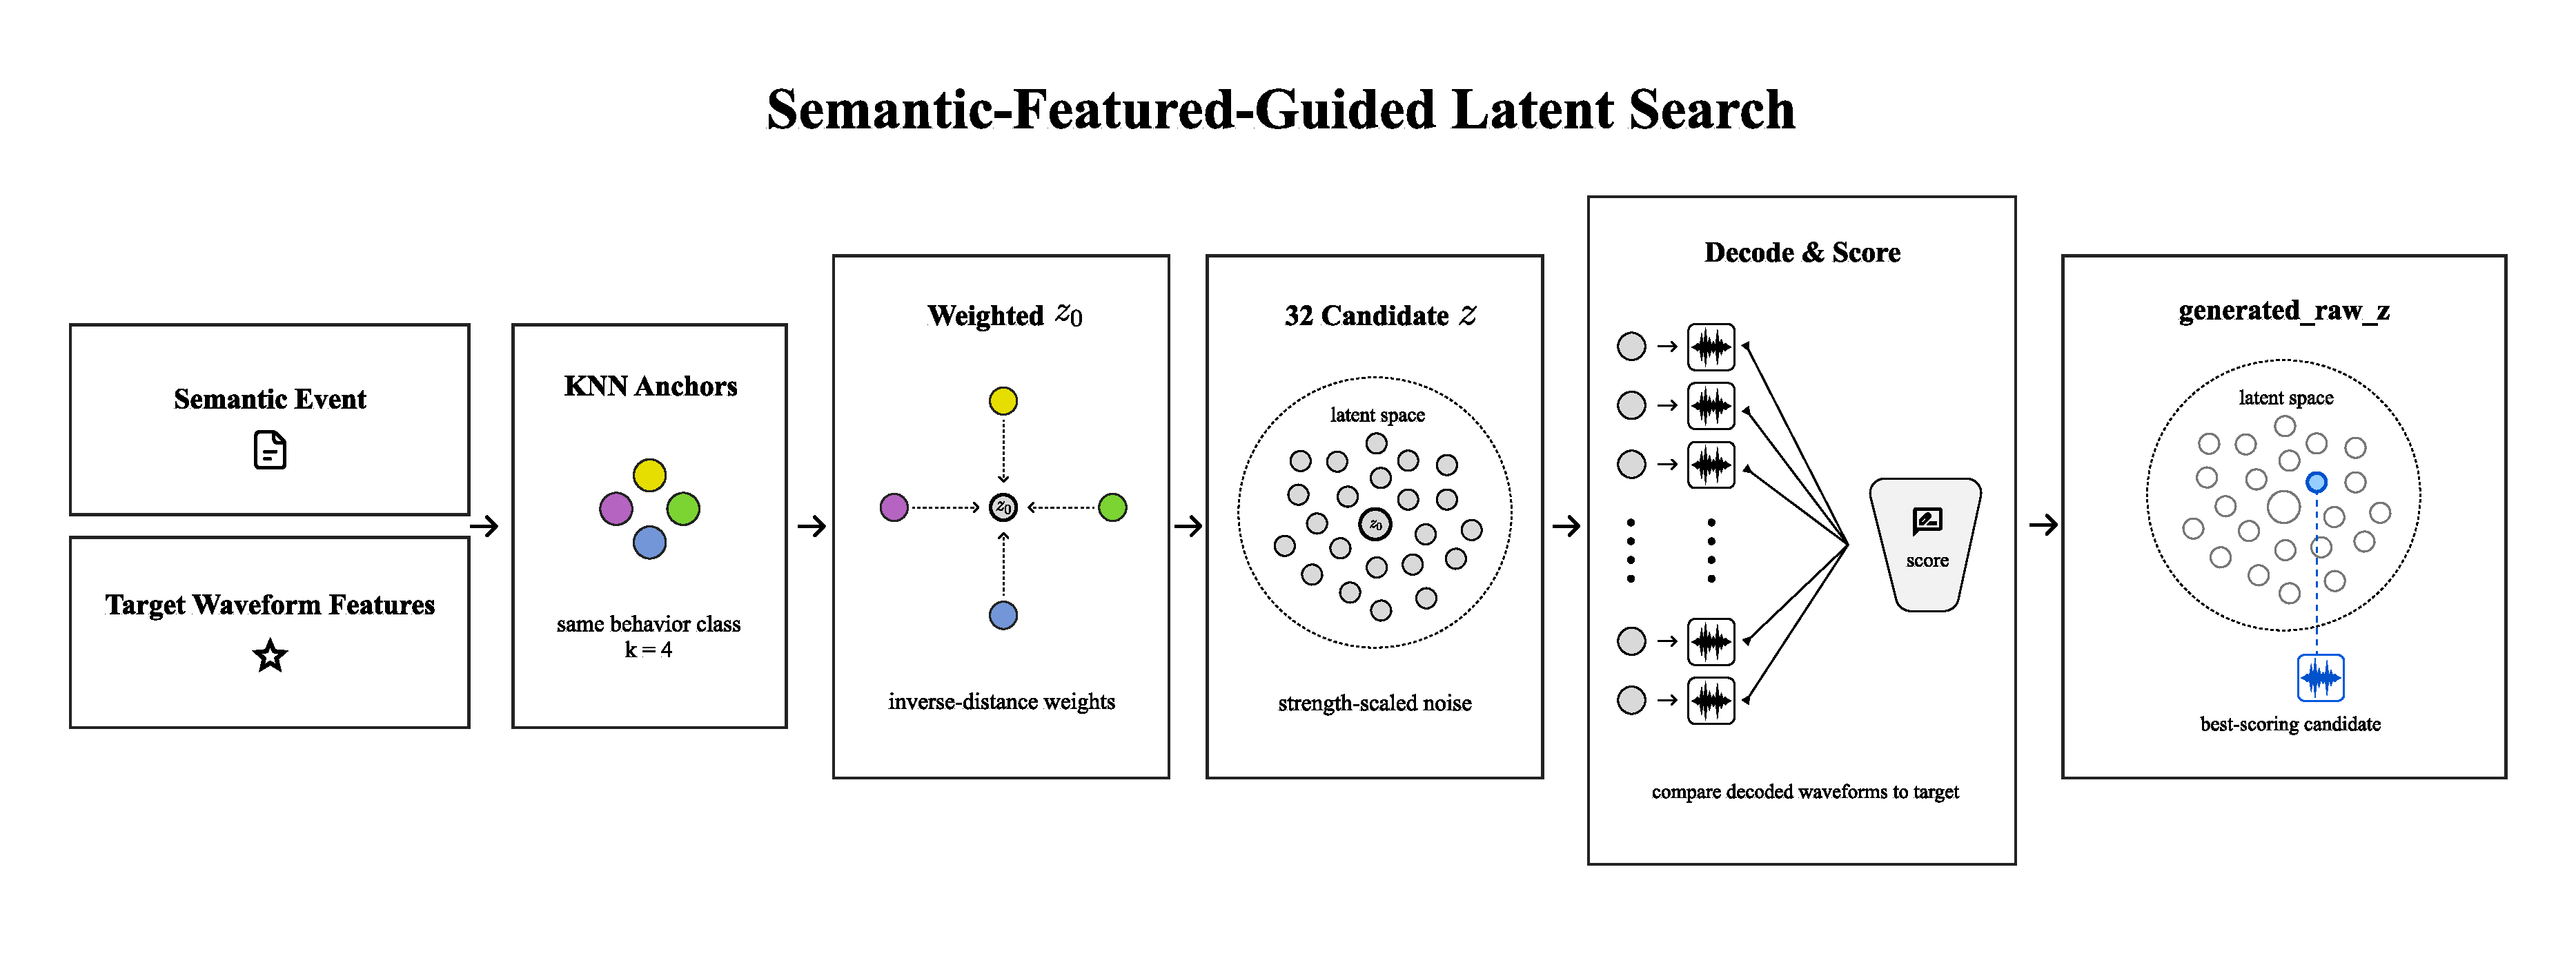
\includegraphics[width=\textwidth]{Figures/latent_search.pdf}
\caption{Semantic-feature-guided latent search.}
\label{fig:latent-search}
\end{figure}

Within the requested behavior class, the system compares the target feature vector against the curated atlas prototypes for that class. The four nearest prototypes are selected as anchors. The user-facing \texttt{prototype\_index} from the event plan biases this anchor selection toward the requested curated example, but the anchors define the local search region rather than the final objective. The objective is the event-derived target vector $\mathbf{t}$. Distances are computed over standardized waveform features with feature-specific weights:

\begin{equation}
D(\mathbf{x}, \mathbf{t}) =
\sqrt{
\sum_m \alpha_m
\left(
\frac{f_m(\mathbf{x}) - t_m}{\sigma_m}
\right)^2
},
\end{equation}

where $f_m(\mathbf{x})$ is feature $m$ of waveform or prototype $\mathbf{x}$, $t_m$ is the semantic target value, $\sigma_m$ is the class-specific feature scale, and $\alpha_m$ is the feature weight.

The selected anchors are weighted by inverse distance. Given anchor latents $\mathbf{z}_i$ and distances $d_i$, the anchor weights and initial latent estimate are

\begin{equation}
w_i =
\frac{1/(d_i+\epsilon)}
{\sum_j 1/(d_j+\epsilon)},
\qquad
\mathbf{z}_0 = \sum_{i=1}^{k} w_i \mathbf{z}_i ,
\end{equation}

with $k=4$. The system then samples 32 candidate latent vectors around $\mathbf{z}_0$. The sampling noise is scaled by the local latent variation of the selected anchors and by the requested event strength:

\begin{equation}
\mathbf{z}_c =
\mathbf{z}_0 +
\boldsymbol{\eta}_c \odot \boldsymbol{\sigma}_{\mathrm{local}}
\sigma_{\mathrm{cand}},
\qquad
\sigma_{\mathrm{cand}} = \lambda(0.45 + 0.75s),
\end{equation}

where $\boldsymbol{\eta}_c$ is standard normal noise, $\boldsymbol{\sigma}_{\mathrm{local}}$ is the local latent standard deviation, $s$ is the event strength, and $\lambda$ is the base candidate noise scale. In this implementation, $\lambda=0.20$, so stronger events search a wider local region around the anchor estimate. Candidate latents are clipped to the class-specific latent range when quantile clipping is enabled.

Each candidate latent vector is decoded by the VAE into a waveform chunk. The scoring step is performed after decoding, so the selection criterion is based on the waveform that the candidate actually generates. For each decoded candidate, the system recomputes the same feature set used in the target representation and compares those features against $\mathbf{t}$. The selected event latent is therefore

\begin{equation}
\mathbf{z}^{*}
=
\arg\min_{\mathbf{z}_c \in \mathcal{Z}_{\mathrm{cand}}}
D\left(F\left(\mathrm{Dec}(\mathbf{z}_c)\right), \mathbf{t}\right),
\end{equation}

where $F$ extracts waveform features and $\mathrm{Dec}$ is the VAE decoder. The best candidate $\mathbf{z}^{*}$ is stored as \texttt{generated\_raw\_z} and decoded into the haptic chunk passed to the timeline mixer.

\section{Event Timeline Mixer}

The event timeline mixer converts the generated event chunks into a fixed two-second haptic response. Each event chunk is produced independently by the VAE decoder, but temporal visual events often contain multiple moments, such as an input action followed by a system response. The mixer preserves this event structure by assigning each generated chunk a duration and position within a shared timeline before producing the final waveform.

The mixer operates at the same sample rate as the VAE, 8 kHz, and produces a final waveform of 16000 samples. Each planned event enters the mixer with a duration hint that has already been mapped to seconds: short, medium, long, or full. If the planned events and gaps fit within the two-second window, those preferred durations are used directly. If they exceed the available time, the mixer first compresses longer events while respecting a minimum event duration, then reduces the inter-event gap if needed, and finally scales all event durations as a fallback.

Each decoded chunk is shaped before placement. The waveform is stretched or held to match the assigned duration using the hold-stretch duration mode. The event strength $s$ is converted to an amplitude gain,

\begin{equation}
g = 0.5 + 0.8s,
\end{equation}

so stronger planned events produce larger waveform amplitudes before clipping. A 10 ms fade is applied at event boundaries to reduce abrupt transitions between silence and vibration.

Timeline placement is determined by event order, timing hints, and alignment rules. Events are separated by a default 0.08-second gap. If the first event is marked as beginning, the sequence starts at the beginning of the two-second response. If the final event is marked as end, or if its role is confirmation, release, notification, or warning, the sequence is aligned so that the event sequence ends near 1.9 seconds. Otherwise, the event sequence is centered in the two-second window. These rules provide deterministic placement while preserving the coarse timing decisions made by the planner.

The mixer combines scheduled chunks additively into the final waveform and clips the result to the configured amplitude range. In the final stimulus generation run, the mixed waveform was clipped to $\pm 3.0$. The output of this stage is still an 8 kHz waveform; the next export stage converts it into a 10 ms interval sequence for ERM playback.

\section{ERM Preprocessing and Export}

The timeline mixer outputs a two-second waveform at 8 kHz, but the study prototype plays discrete motor drive values rather than audio-rate waveform samples. The export stage therefore converts the mixed waveform into a 10 ms interval sequence with 200 values over the same two-second duration. This sequence represents the intended drive envelope for the actuator, not an audio signal.

The ERM preprocessing stage then converts the 10 ms sequence into a hardware-ready 20 ms interval sequence with 100 values. The conversion uses peak-hold resampling from 10 ms to 20 ms so that short peaks are preserved when the sequence is downsampled. Low values below the motor threshold are removed, and the remaining values are remapped with a gamma curve into a bounded drive range. The preprocessing also extends very short nonzero pulses and applies short attack and release smoothing so that events remain perceivable on an ERM motor.

This preprocessing is important because ERM motors have physical inertia and a practical activation threshold. Very brief or low-amplitude changes in a raw sequence may not produce reliable tactile sensations, while abrupt changes can feel inconsistent across stimuli. The preprocessing stage makes the generated sequence more compatible with the actuator while preserving the event timing produced by the earlier pipeline stages.

All five methods compared in the user study use this same export and ERM preprocessing pipeline. Random Noise, Random VAE, HapticGen, Direct LLM Pattern, and Semantic VAE each produce a two-second, 10 ms interval sequence before preprocessing, and each is converted into the same 20 ms interval ERM-ready format. The user study therefore compares the haptic generation methods under a shared playback representation rather than under method-specific actuator processing.

Together, these stages define the final generation method evaluated in this thesis. The system represents visual transitions as semantic haptic events, uses the behavior atlas to guide generation in the VAE latent space, composes generated chunks into a fixed temporal response, and exports that response through a shared ERM playback format. The next chapter describes how this method was evaluated against alternative generation baselines in a controlled user study.
